\begin{center}
    \rule{\textwidth}{1pt} \\[0.5cm]
    {\Huge \bfseries ANNEXE} \\[0.4cm]
    \rule{\textwidth}{1pt}
\end{center}

\section*{Échantillonnage (\ref{section-echantillonnage})}
\phantomsection
\label{preuve-echantillonnage}

Le passage au numérique demande de ne conserver que certaines valeurs isolées du signal. Nous devons alors introduire la notion de \textbf{distribution de Dirac}. Dans le cadre de notre étude, nous utiliserons une définition alternative \cite{dirac} , plus faible que la définition usuelle du Dirac. Cette définition plus intuitive est parfaitement suffisante pour l'utilisation que l'on en fera et ne fait pas appel à la théorie de la mesure.

Soit $(f_\alpha)_{\alpha \in \mathbb{\mathbb{R}+}}$ la famille de fonctions définies par :
\begin{align*}
    f_\alpha : t \mapsto \left\{ \begin{array}{cl} \frac{1}{2\alpha} & \text{si} \ t \in [-\alpha;\alpha] \\ 0 &  \text{sinon} 
\end{array} \right.
\end{align*}

On définit l'action du Dirac $\delta$ sur une fonction $g$, continue en $0$, par :
\begin{align*}
    \int_{-\infty}^{+\infty} g(t) \delta(t) dt \coloneqq \lim_{\alpha \to 0}  \int_{-\infty}^{+\infty} g(t) f_\alpha(t) dt
\end{align*}
Soit $\alpha > 0$,
\begin{align*}
    \int_{-\infty}^{+\infty} f_\alpha(t) dt = \int_{-\alpha}^{\alpha} \frac{1}{2\alpha} dt = \frac{1}{2\alpha} \int_{-\alpha}^{\alpha} dt = 1
\end{align*}

\begin{figure}[H]
    \caption{$f_\alpha$ pour $\alpha = 1, \tfrac{1}{2}, \tfrac{1}{4}$}
    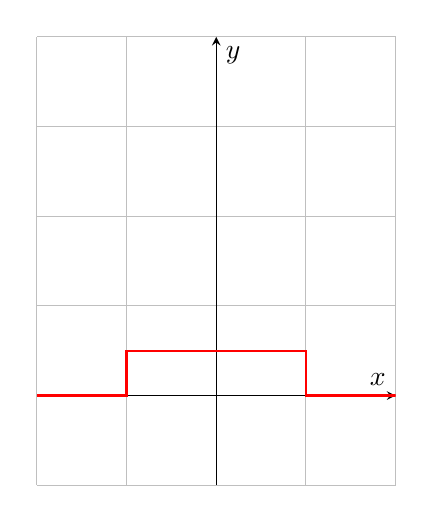
\begin{tikzpicture}[scale = 1]
        \begin{axis}[
            axis lines = middle,
            unit vector ratio={1 1},
            xlabel = {$x$},
            ylabel = {$y$},
            ymin = -0.5, ymax = 2,
            xmin = -1, xmax = 1,
            grid = both,
            xticklabels = {,,},
            yticklabels = {,,},
            tick style = {draw=none}
        ]
        \addplot [color=red, thick] coordinates {
            (-1, 0) 
            (-0.5, 0) 
            (-0.5, 0.25) 
            (0.5, 0.25) 
            (0.5, 0) 
            (1, 0)
        };
        \end{axis}
    \end{tikzpicture}
    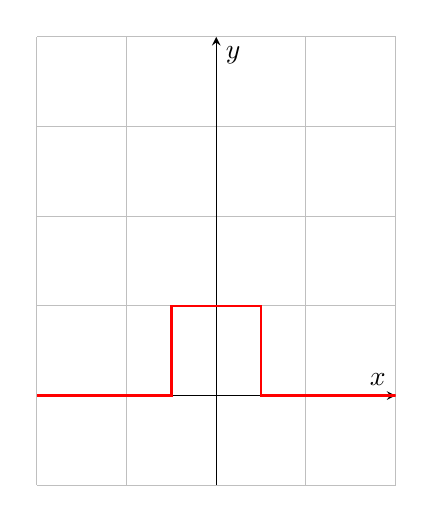
\begin{tikzpicture}[scale = 1]
        \begin{axis}[
            axis lines = middle,
            unit vector ratio={1 1},
            xlabel = {$x$},
            ylabel = {$y$},
            ymin = -0.5, ymax = 2,
            xmin = -1, xmax = 1,
            grid = both,
            xticklabels = {,,},
            yticklabels = {,,},
            tick style = {draw=none}
        ]
        \addplot [color=red, thick] coordinates {
            (-1, 0) 
            (-0.25, 0) 
            (-0.25, 0.5) 
            (0.25, 0.5) 
            (0.25, 0) 
            (1, 0)
        };
        \end{axis}
    \end{tikzpicture}
    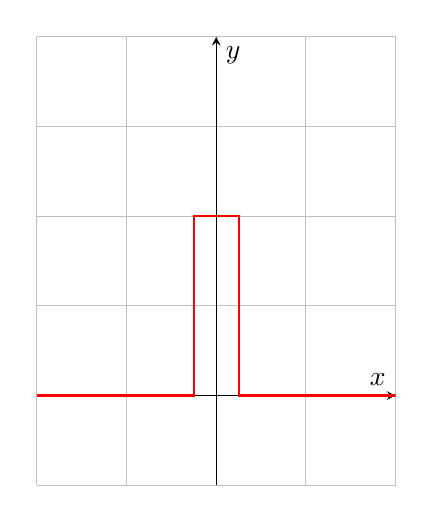
\begin{tikzpicture}[scale = 1]
        \begin{axis}[
            axis lines = middle,
            unit vector ratio={1 1},
            xlabel = {$x$},
            ylabel = {$y$},
            ymin = -0.5, ymax = 2,
            xmin = -1, xmax = 1,
            grid = both,
            xticklabels = {,,},
            yticklabels = {,,},
            tick style = {draw=none}
        ]
        \addplot [color=red, thick] coordinates {
            (-1, 0) 
            (-0.125, 0) 
            (-0.125, 1) 
            (0.125, 1) 
            (0.125, 0) 
            (1, 0)
        };
        \end{axis}
    \end{tikzpicture}
\end{figure}


En appliquant la définition de l'action du Dirac sur la fonction constante $g = 1$, on obtient :
\begin{align*}
    \int_{-\infty}^{+\infty} \delta(t) dt = \lim_{\alpha \to 0^+} \int_{-\infty}^{+\infty}f_\alpha(t)dt = \lim_{\alpha \to 0^+} 1 = 1
\end{align*}

En traitement du signal, on considère souvent abusivement que $\delta$ est une fonction réelle, valant 0 partout sauf en 0 où elle vaut \og +$\infty$ \fg,  mais il s'agit bien d'une distribution caractérisée par :

\begin{description}
    \item[Sa concentration] : $\forall t \neq 0, \delta(t) = 0$
    \item[Sa masse] : $\int_{-\infty}^{+\infty}\delta(t)dt = 1$
\end{description}

On fera également attention à garder à l'esprit que la notation sous forme d'intégrale impropre sur $\mathbb{R}$ faisant intervenir le Dirac dans l'intégrande fait toujours référence à la définition de l'action du Dirac sous forme de limite et ne pose aucun problème de convergence du moment que $g$ est intégrable au voisinage de 0.

L'intérêt, pour le traitement du signal, de la distribution de Dirac est sa capacité à isoler une valeur ponctuelle d'un signal. En effet, si on définit de la même manière, l'action du Dirac $\delta(t - t_0)$, centré en $t_0$, par l'identité $\int_{-\infty}^{+\infty} g(t) \delta(t-t_0) dt = \lim_{\alpha \to 0+} \int_{-\infty}^{+\infty} g(t) f_{\alpha}(t-t_0) dt$, alors, on obtient, pour toute fonction $g$ continue en $t_0$, la relation suivante :
\begin{align*}
    \int_{-\infty}^{+\infty} g(t) \delta(t-t_0) dt = g(t_0)
\end{align*}

\begin{proof}
    \vspace{0.2cm}
    
    Soit $g$ une fonction continue en $t_0 \in \mathbb{R}$, on a :
    \begin{align*}
        \int_{-\infty}^{+\infty} g(t) \delta(t - t_0) dt = \lim_{\alpha \to 0+} \int_{-\infty}^{+\infty} g(t) f_{\alpha}(t - t_0) dt
    \end{align*}
    Soit $\alpha > 0$,
    \begin{align*}
        \int_{-\infty}^{+\infty} g(t) f_{\alpha}(t - t_0) dt &= \int_{t_0 - \alpha}^{t_0 + \alpha} \frac{g(t)}{2\alpha} dt \\
        &= \frac{1}{2 \alpha} \int_{t_0 - \alpha}^{t_0 + \alpha} g(t) dt \\
        &= \frac{1}{2 \alpha} \left( \int_{t_0 - \alpha}^{t_0 + \alpha} g(t_0) dt + \int_{t_0 - \alpha}^{t_0 + \alpha} \left( g(t) - g(t_0) \right) dt \right) \\
        &= g(t_0) + \frac{1}{2 \alpha} \int_{t_0 - \alpha}^{t_0 + \alpha} \left( g(t) - g(t_0) \right) dt
    \end{align*}
    Or, 
    \begin{align*}
        \left| \frac{1}{2 \alpha} \int_{t_0 - \alpha}^{t_0 + \alpha} \left( g(t) - g(t_0) \right) dt \right| &\leq \frac{1}{2 \alpha} \int_{t_0 - \alpha}^{t_0 + \alpha} \left| g(t) - g(t_0) \right| dt \\
        &\leq \sup_{t \in \left[ t_0 - \alpha ; t_0 + \alpha \right]} \left| g(t) - g(t_0) \right| \to 0 \quad \text{par continuité de g en $t_0$}
    \end{align*}

    Ainsi, on a bien $\lim_{\alpha \to 0+} \int_{-\infty}^{+\infty} g(t) f_{\alpha}(t - t_0) dt = g(t_0)$.

\end{proof}

Pour obtenir un échantillonnage d'un signal, il faut réaliser plusieurs extractions de valeurs à l'aide du Dirac. Il est alors pertinent d'introduire le \textbf{peigne de Dirac} de période $T$, noté $\Sha_{T}$ :
\begin{align*}
    \Sha_{T}(t) = \sum_{n\in\mathbb{Z}} \delta(t - nT)
\end{align*}

\begin{figure}[H]
    \begin{center}
    \caption{Peigne de Dirac de période $T$}
    \begin{tikzpicture}[scale=1.5]
        \draw[->] (-3,0) -- (3,0) node[right] {$t$};
        \draw[->] (0,-0.5) -- (0,1.5) node[above] {$\Sha_{T}(t)$};
        \foreach \x in {-2.5, -2, ..., 2.5} {
            \draw[-, blue, thick] (\x, 0) -- (\x, 1);
            \draw[dashed, blue, thick] (\x, 1) -- (\x, 1.5);
        }
        \draw[<->] (1, -0.15) -- (1.5, -0.15) node[midway, below, font=\tiny] {$T$};
    \end{tikzpicture}
    \end{center}
\end{figure}

Le signal échantillonné $s_e(t)$ est alors modélisé par le produit du signal analogique $s(t)$ et du peigne de Dirac $\Sha_{T}$:
\begin{align*}
    s_e(t) = s(t) \cdot \Sha_{T}(t) = \sum_{n\in\mathbb{Z}} s(nT) \delta(t - nT)
\end{align*}

\pagebreak

\section*{Transformée de Fourier Discrète Inverse (\ref{section-TFD})}
\phantomsection
\label{preuve-TFDI}

$$TFDI(TFD(x_n)) = x_n$$
\begin{proof}
    Soit $(x_0,x_1,...,x_{N-1}) \in \mathbb{C}^N$. Soit $0 \leq n < N$.

    \begin{align*}
        TFDI(TFD(x_n))&=\dfrac{1}{N} \sum_{k=0}^{N-1} \left(\sum_{m=0}^{N-1} x_m e^{-i \frac{2\pi}{N} km}\right) e^{i \frac{2 \pi}{N}kn} \\
        &= \dfrac{1}{N} \sum_{m=0}^{N-1} x_m \left( \sum_{k=0}^{N-1} e^{-i \frac{2\pi}{N} k(m-n)} \right)
    \end{align*}
    Posons :
    $$S_N \coloneq \sum_{k=0}^{N-1}e^{-i \frac{2\pi}{N} k(m-n)}$$
    On remarque que $S_N$ est une somme partielle d'une suite géométrique de raison $q = e^{-i \frac{2\pi}{N} (m-n)}$.
    \begin{description}
        \item[Si $n=m$, ] $q = e^0 = 1 \implies S_N = \sum_{k=0}^{N-1} 1 = N$  
        \item[Si $n\neq m$, ] $S_N=\frac{1-q^N}{1-q}$ or, $q^N = e^{-i2\pi(m-n)} = 1$ car $m-n\in \mathbb{Z}$ donc $S_N = 0$ 
    \end{description}
    $$\implies TFDI(TFD(x_n)) =\dfrac{1}{N}\sum_{m=0}^{N-1}x_m \cdot N \delta_{nm} = \dfrac{1}{N}x_n\cdot N = x_n$$
\end{proof}

\pagebreak

\section*{Exemple Cooley-Tukey (\ref{section-cooley-tukey})}
\phantomsection
\label{exemple-cooley}

Lorsqu'on atteint l'étape de combinaison ("le papillon"), on considère les FFT des sous-signaux pairs ($E$) et impairs ($O$) de taille $n=4$ déjà calculées. 
De même avant la première boucle on a $\alpha$ = 1.

\subsubsection*{Itération 1 : $k=0$}
\begin{itemize}
    \item \textbf{Calcul des composantes :}
    \begin{itemize}
        \item $X_0 = E[0] + \alpha \times O[0] = E[0] + 1 \times O[0]$
        \item $X_4 = E[0] - \alpha \times O[0] = E[0] - 1 \times O[0]$
    \end{itemize}
    \item \textbf{Mise à jour du facteur tournant :}
    \begin{itemize}
        \item $\alpha \leftarrow \alpha \times \omega = 1 \times \omega = \omega$
    \end{itemize}
\end{itemize}

\subsubsection*{Itération 2 : $k=1$}
\begin{itemize}
    \item \textbf{Calcul des composantes :}
    \begin{itemize}
        \item $X_1 = E[1] + \alpha \times O[1] = E[1] + \omega \times O[1]$
        \item $X_5 = E[1] - \alpha \times O[1] = E[1] - \omega \times O[1]$
    \end{itemize}
    \item \textbf{Mise à jour du facteur tournant :}
    \begin{itemize}
        \item $\alpha \leftarrow \alpha \times \omega = \omega \times \omega = \omega^2$
    \end{itemize}
\end{itemize}

Le processus continue ainsi pour $k=2$ et $k=3$ afin de compléter les 8 éléments du signal final $X$.

\begin{flushleft}

\renewcommand{\arraystretch}{1.5}
\[
\begin{array}{|l|l|l|}
\hline
\textbf{Étape} & \textbf{Calculs des sorties } X & \textbf{Mise à jour de } \alpha \\
\hline
k=2 & X_2 = E[2] + \omega^2 \cdot 0[2], \quad X_6 = E[2] - \omega^2 \cdot 0[2] & \alpha \leftarrow \omega^2 \cdot \omega \\
\hline
k=3 & X_3 = E[3] + \omega^3 \cdot 0[3], \quad X_7 = E[3] - \omega^3 \cdot 0[3] & \alpha \leftarrow \omega^3 \cdot \omega \\
\hline
\end{array}
\]

\end{flushleft}

On reconstruit $X = (X_0, X_1, X_2, X_3, X_4, X_5, X_6, X_7)$.

\pagebreak

\section*{Compilation à la volée (\ref{section-approche-iterative})}
\phantomsection
\label{compilation-jit}

On peut observer graphiquement que notre version itérative est plus rapide en moyenne que la version récursive de la FFT mais elles restent toutes les deux très loin de l'implémentation de référence de numpy. Cet écart est dû, dans une moindre mesure, à des optimisations supplémentaires mises en oeuvre dans l'implémentation numpy, mais surtout au fait que la librairie numpy fait appel à du code C compilé là où notre implémentation en pur python est simplement interprétée.

Pour pallier ce problème, une solution simple serait de réécrire tout notre code en C, néanmoins, en python toujours, il est possible de faire un compromis consistant en la compilation à la volée (\textit{just in time compilation}\cite{wiki-jit}). En temps normal, l'interpréteur python traduit dans un premier temps le code python en bytecode, qui sera ensuite exécuté par une machine virtuelle. En utilisant une librairie de compilation à la volée, par exemple numba, le bytecode produit est compilé, s'il est jugé que cela apporterait un gain de performance, en langage machine.

Avec cette amélioration, nos deux implémentations de Cooley-Tukey se rapprochent des performances de l'implémentation de numpy. On peut en outre remarquer que l'implémentation itérative semble plus bénéficier de la compilation à la volée.

\begin{figure}[H]
    \centering
    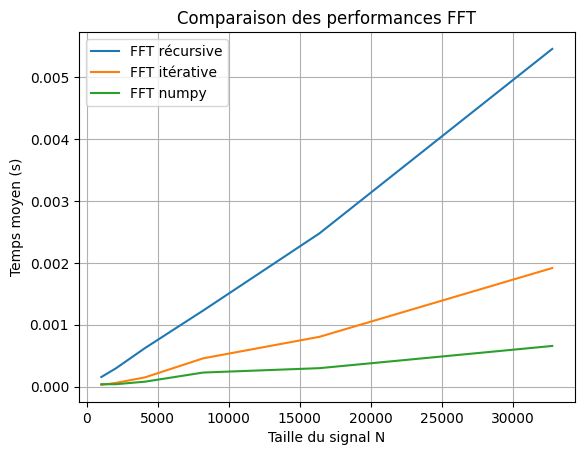
\includegraphics[width=0.6\textwidth]{images/FFT_performances_compilees.png}
    \caption{Temps de calcul moyen en fonction de la taille du signal pour différentes FFT, avec compilation à la volée.}
\end{figure}

\pagebreak

\section*{Interprétation du spectre (\ref{section-spectre-fft})}
\phantomsection
\label{preuve-spectre-fft}
Les basses fréquences sont situées dans les coins du spectre. 

\begin{proof}
    En effet, les fréquences discrètes étant périodiques, on peut les représenter sur un tore discret. Ainsi, les coins ne sont pas proches sur le spectre visuellement mais sont mathématiquement adjacents grâce à leur périodicité modulo $N$ et $M$. On peut alors définir une distance sur ce tore en tirant parti de la symétrie modulo $N$ : $d_N(x, y) = \min(|x - y| \pmod N, N - (|x - y| \pmod N))$ (pareil dans l'autre direction avec $M$). Ainsi, on peut mesurer la distance d'un point par rapport à l'origine en faisant $d_N(k,0)=\min(k,N-k)$.
\begin{figure}[H]
    \centering
    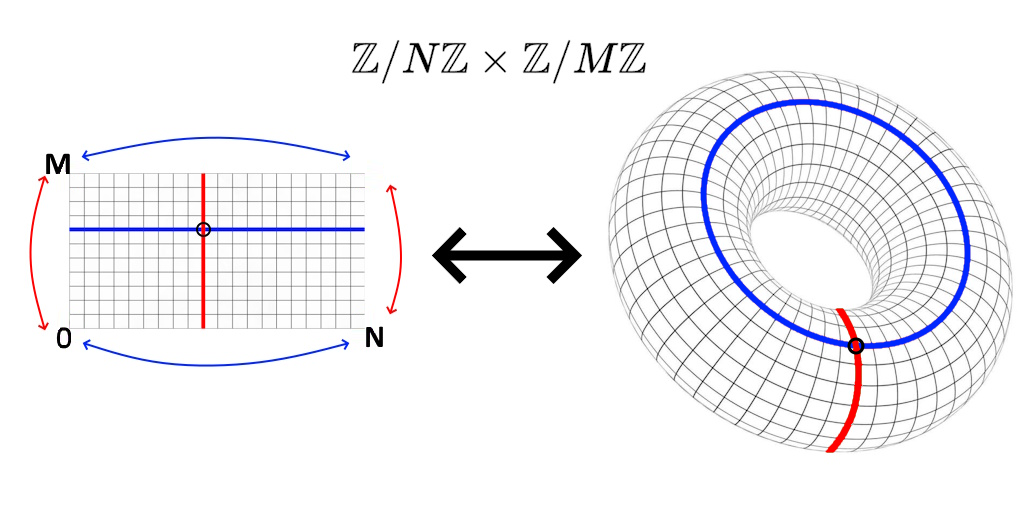
\includegraphics[width=0.75\textwidth]{images/Tore.png}
    \caption{Représentation visuelle en tore}
\end{figure}
Soient $k \in \{0, \dots, M-1\}$ et $l \in \{0, \dots, N-1\}$ \\
Posons $\varphi_{k,l}: \mathbb{Z}/N\mathbb{Z} \times  \mathbb{Z}/M\mathbb{Z} \to \mathbb{C}$ telle que $\varphi_{k,l}(n,m)=\exp(-2i\pi (\frac{kn}{N} + \frac{lm}{M}))$
Nous pouvons alors étudier le taux d'accroissement entre deux fréquences discrètes.
$$\frac{\varphi_{k,l}(n+1,m)}{\varphi_{k,l}(n,m)} = \frac{\exp(-2i\pi (\frac{k(n+1)}{N} + \frac{lm}{M}))}{\exp(-2i\pi (\frac{kn}{N} + \frac{lm}{M}))} = e^{\frac{-2i\pi k}{N}}$$
Ainsi, \\
$d_N(k,0) \ll N \implies |\frac{2\pi k}{N}|\ll 1 \implies e^{\frac{-2i \pi k}{N}} \approx 1 \implies \varphi_{k,l}(n+1,m) \approx \varphi_{k,l}(n,m)$ \\
$k \approx \frac{N}{2} \implies e^{\frac{-2i \pi k}{N}} \approx -1 \implies \varphi_{k,l}(n+1,m) \approx -\varphi_{k,l}(n,m)$
Plus la distance $d_N(k,0)$ est faible, moins la fonction présente d'oscillations, ce qui traduit la présence de basses fréquences. À l'inverse, plus $k$ est proche de $\frac{N}{2}$, plus la fonction oscille rapidement, ce qui correspond à des hautes fréquences.Par un raisonnement analogue sur l'accroissement dans la seconde direction (selon l'indice $l$ et la dimension $M$), on montre que les variations spatiales suivent la même logique.En conclusion, les fréquences les plus faibles (les composantes continues et lentes du signal) se concentrent autour de l'origine et, par périodicité modulo $N$ et $M$, se retrouvent également dans les quatre coins du spectre discret.
\end{proof}

\pagebreak

\section*{Compression avec la FFT (\ref{section-spectre-fft})}
\phantomsection
\label{preuve-compression-fft}

\begin{proof}
    Soit $f$ une image de taille $M \times N$, représentée par une matrice de pixels où $f(n, m) \in \mathbb{C}$ est l'intensité du pixel à la position $(n, m)$. On étudie le spectre de l'image (appartenant à $\mathbb{C}^{M\times N}$) par une transformée de Fourier discrète (FFT).

    On considère le produit scalaire standard sur cet espace : 
    $$ 
    \langle f,g \rangle = \sum_{n=0}^{M-1}\sum_{m=0}^{N-1}f(n,m)\overline{g(n,m)}
    $$
    On définit une distance sur cet espace en tirant parti de la symétrie modulo $M$ (respectivement $N$) : $d_M(x, y) = \min(|x - y| \pmod M, M - (|x - y| \pmod M))$. Ainsi, on mesure la distance d'un point par rapport à l'origine en faisant $d_M(k,0)=\min(k,M-k)$.

    Soient $k \in \{0, \dots, M-1\}$ et $l \in \{0, \dots, N-1\}$. Les fonctions $\varphi_{k,l}: \mathbb{Z}/M\mathbb{Z} \times \mathbb{Z}/N\mathbb{Z} \to \mathbb{C}$ telles que $\varphi_{k,l}(n,m)=\exp\left(-2i\pi \left(\tfrac{kn}{M} + \tfrac{lm}{N}\right)\right)$ forment une base orthogonale de $\mathbb{C}^{M\times N}$.
    
    Posons $R \in [0,1]$, le ratio de conservation des fréquences pour l'image. Comme $\mathbb{C}^{M\times N}$ est un espace vectoriel de dimension finie, on peut écrire la décomposition unique :
    $$
    f = f_R + h \quad \text{avec } f_R \in V_R, \, h \in {V_R}^{\perp}
    $$
    
    où $V_R = \text{Vect} \left\{\varphi_{k,l} \mid d_M(k,0) \leq RM \text{ et } d_N(l,0) \leq RN\right\}$.

    Soit $g \in V_R$,
    $$
    f-g=(f_R+h)-g=(f_R-g)+h
    $$
    or, $f_R-g \in V_R$ et $h \in V_R^{\perp}$, donc $\langle f_R-g, h \rangle = 0$. On a alors, d'après le théorème de Pythagore : 
    \begin{align*}
        \lVert f-g \rVert^2 &= \lVert f_R-g \rVert^2 + \lVert h \rVert^2 \\
                            &\implies \lVert f-g \rVert^2 \geq \lVert h \rVert^2 \\
                            &\implies (\lVert f-g \rVert^2 = \lVert h \rVert^2 \iff g = f_R) \\
                            &\implies \lVert f-f_R \rVert^2 = \min_{g \in V_R} \lVert f-g \rVert^2
    \end{align*}

    Ainsi, la fonction minimisant l'erreur $\lVert f-f_R \rVert^2$ est la fonction g qui est donc le projeté orthogonal sur le sous-espace vectoriel $V_R$ formé par les $\varphi_{k,l}$ ayant leurs $k$ et $l$ proches de l'origine. C'est donc l'hyperplan formé par les fréquences les plus basses. Il faut ainsi conserver les fréquences faibles pour compresser une image à l'aide d'une FFT.
    
\end{proof}

\pagebreak

\section*{Base orthonormale pour la DCT (\ref{section-DCT})}
\phantomsection
\label{preuve-base-DCT}

Les $ e_k(n) = \alpha_k \cos\left(\frac{\pi}{N}\left(n+\frac{1}{2}\right)k\right),\quad k=0,\dots,N-1 $ forment une base orthonormale pour le produit scalaire usuel sur $\mathbb{R}^N$.
\begin{proof}
    On considère le produit scalaire usuel sur $\mathbb{R}^N$ :
    $ \langle x,y\rangle = \sum_{n=0}^{N-1} x_ny_n $
    On calcule :
    $$
        \langle e_k,e_l\rangle = \alpha_k \alpha_l \sum_{n=0}^{N-1} \cos\left(\frac{\pi}{N}\left(n+\frac{1}{2}\right)k\right) \cos\left(\frac{\pi}{N}\left(n+\frac{1}{2}\right)l\right)
    $$

        On remarque alors que $\sum_{n=0}^{N-1} \cos\left(\theta\left(n + \frac{1}{2}\right)\right) = \frac{\sin(N\theta/2)}{2\sin(\theta)}$, d'où :
    \begin{align*}
        \langle e_k,e_l\rangle
        &= \frac{\alpha_k \alpha_l}{2} \left( \frac{\sin(N(\theta_k - \theta_l))}{2\sin((\theta_k - \theta_l)/2)} + \frac{\sin(N(\theta_k + \theta_l))}{2\sin((\theta_k + \theta_l)/2)} \right) \\
        &= \frac{\alpha_k \alpha_l}{4} \left( \frac{\sin(\pi(k-l))}{\sin(\pi(k-l)/2N)} + \frac{\sin(\pi(k+l))}{\sin(\pi(k+l)/2N)} \right)
    \end{align*}
\begin{itemize}
    \item Si $k \neq l$, alors $\langle e_k,e_l\rangle = \sin(\pi(k-l)) = \sin(\pi(k+l)) = 0$
    \item Si $k=l \neq 0$, le premier terme vaut $2N$ et le second est nul :
    $\langle e_k,e_k\rangle = \frac{\alpha_k^2}{4} 2N = \frac{1}{2N}2N= 1$
    \item Si $k=l=0$, les deux termes valent $2N$ par continuité en 0 :
    $\langle e_0,e_0\rangle = \frac{\alpha_0^2}{4} (2N + 2N) = 1$
\end{itemize}

    Ainsi, la famille $(e_k)$ forme une base orthonormale de $\mathbb{R}^N$.
\end{proof}

\pagebreak

\section*{Transformée en Conisus Discrète Inverse (\ref{section-DCT})}
\phantomsection
\label{preuve-IDCT}

$$IDCT(DCT(x_n)) = x_n$$
\begin{proof}
    On a, par définition,
    \begin{align*}
        X_k = \alpha_k\sum_{m=0}^{N-1}x_m\cos \left[\frac{\pi}{N}\left(m+\frac{1}{2}\right)k\right] \\
        x_n = \sum_{k=0}^{N-1}\alpha_k X_k\cos \left[\frac{\pi}{N}\left(n+\frac{1}{2}\right)k\right]\\
    \end{align*}
    On développe, 
    \begin{align*}
        IDCT(DCT(x_n))&=\sum_{k=0}^{N-1}\alpha_k \left(\alpha_k\sum_{m=0}^{N-1}x_m\cos \left[\frac{\pi}{N}\left(m+\frac{1}{2}\right)k\right]\right)\cos \left[\frac{\pi}{N}\left(n+\frac{1}{2}\right)k\right]\\
        &=\sum_{k=0}^{N-1}\left(\alpha_k^2\sum_{m=0}^{N-1}x_m\cos \left[\frac{\pi}{N}\left(m+\frac{1}{2}\right)k\right]\right)\cos \left[\frac{\pi}{N}\left(n+\frac{1}{2}\right)k\right]\\
        &=\sum_{m=0}^{N-1}x_m\left(\sum_{k=0}^{N-1}\alpha_k^2\cos \left[\frac{\pi}{N}\left(m+\frac{1}{2}\right)k\right]\cos \left[\frac{\pi}{N}\left(n+\frac{1}{2}\right)k\right]\right)\\
        &=\sum_{m=0}^{N-1}x_m\left(\sum_{k=0}^{N-1}\left(\alpha_k\cos \left[\frac{\pi}{N}\left(m+\frac{1}{2}\right)k\right]\right)\left(\alpha_k\cos \left[\frac{\pi}{N}\left(n+\frac{1}{2}\right)k\right]\right)\right) \\
    \end{align*}
    Posons $e_i(k) =\alpha_k\cos\left[\frac{\pi}{N}\left(i+\frac{1}{2}\right)k\right], e_i=(e_i(0),e_i(1), \dots ,e_i(N-1)) \in \mathbb{R}^N$, alors,
    \begin{align*}    
        IDCT(DCT(x_n)) &=\sum_{m=0}^{N-1}x_m\left(\sum_{k=0}^{N-1}e_m(k)e_n(k)\right) \\
        &=\sum_{m=0}^{N-1}x_m\langle e_m,e_n\rangle =\sum_{m=0}^{N-1}x_m\delta_{m,n} = x_n
    \end{align*}
\end{proof}